The study of the role of financial market frictions for the dynamics of the macro-economy
has a long tradition that started well before the 2008 financial crisis. Bernanke and Gertler
(1989) and Kiyotaki and Moore (1997) are two well-known studies that incorporate financial
frictions in general equilibrium models and became the standard references for this literature.
However, before the 2008 financial crisis, the mainstream approach to the study of the
macro-economy abstracted from financial frictions.

This was, in part, motivated by the view that, although markets are clearly incomplete, 
the importance of financial frictions for the dynamics of the macro-economy is somewhat negligible. 
Based on this view, it became preferable to use models with complete markets because they allow 
for simpler analytical characterization. These models featured many frictions such as sticky prices, 
sticky wages, adjustment costs in investment, variable capital utilization, matching frictions in the labor
market, but not financial frictions.

Prior to the 2008 financial crisis, the main idea was that financial frictions could make the real
impact of a shock bigger (amplification) or smaller (dampening). However, financial frictions
are not the initial ‘cause’ of macroeconomic expansions and contractions: something else has
to happen first in the nonfinancial sector. The analysis of financial shocks as a ‘source’ of
macroeconomic fluctuations has received more attention after the 2008 financial crisis.

\begin{itemize}
    \item The financial crisis can be analysed from many different angles
    (labor: banker’s pay and incentives, intl macro: savings glut,
    micro: coordination failures/bank runs, political economy).
    \item We are going to model one mechanism that gives a role for
    asset prices in the transmission of shocks.
    \item This mechanism gives an answer to the question: why were
    the real effects of the bursting of the housing bubble so big?
\end{itemize}

\section{Credit markets and asymmetric information}

Fundamental problem that borrowers have more information
about (and more control over) the projects they undertake
than the lenders who finance them.

WE assume that lender cannot verify the outcome of an investment project
without some monitoring cost.

Known as the \textit{costly state verification} problem.

Leads to a positive external finance premium.

\subsection{Entrepreneurs}
We assume they are \textit{risk neutral},and die with probability $1-\gamma$,
so that they never accumulate enough net worth to become self-financing.

They borrow money, in addition to using their net worth, to acquire capital.

They also supply some labor to the general labor market.

\subsubsection{Idiosyncratic risk}
Entrepreneurs can do a “project” in every period, which yields
a total nominal payoff of
\[\omega R^k Q K\]
if $K$ units of capital are used. $Q$ is the price of one unit of capital.

Hence, $\omega R^k$ is the gross nominal return on capital, where $\omega$ is the
firm-specific component and $R^k$ is the aggregate component(same for all firms).

$\omega$ is drawn from a continuous distribution $F(x), f(x)$ and an expectation $\mathbb{E}[\omega] =1$.

\textit{Ex ante}, either the entrepreneur nor the lender observe $\omega $ befor undertaking project;
\textit{ex post}, the entrepreneur knows $\omega$, the lender would have to pay a monitoring cost, 
a friction $\mu$ of ex post project payoff to verify $\omega$.

\subsubsection{Borrowing decision and contract offered by lender}
Suppose the entrepreneur has net worth $N$ at the beginning, price of capital goods is $Q$.

For entrepreneurs to acquire $K$ units of capital, they need to borrow $QK-N$ once net worth has been used.

If the extrepreneur's idiosyncratic shock is $\omega $, the total project payoff is $\omega R^{k}QK$.

The financial contract we consider specifies a threshold $\bar{\omega }$ such that:
\begin{enumerate}
    \item If $\omega \geq \bar{\omega }$, then a fixed amount $\overline{\omega}R^k QK$ is repaid.
    \item If $\omega < \bar{\omega }$, then the borrower defaults. and after the lender determined $\omega $,
    the borrower is seized $(1-\mu) \omega R^k QK$.
\end{enumerate}

This type of contract is known as \textit{risky debt} and can be shown
to contain a contract that is optimal from the borrower’s
pespective (see micro/mechanism design class).

\subsubsection{Lender's problem}
Suppose the lender is able to diversify lending across a large
representative sample of entrepreneurs with net worth $N$.

As entrepreneurs’ idiosyncratic draws are independent, the law
of large numbers applies and the actual return on lending
amount $QK-N$ is:
\[\left(\overline{\omega}(1-F(\overline{\omega})) + (1-\mu) \int_{0}^{\overline{\omega}} \omega f(\omega) d \omega\right)R^k QK\]

Suppose the lender’s outside option for lending is to earn a
risk-free interest $R$. Assuming perfect competition between
lenders, we get that the above must equal $R(QK-N)$.

\subsubsection{Division of gross profits}
Define the lender’s gross share of aggregate revenues (before
monitoring costs) as
\[
\Gamma(\overline{\omega}) = \int_{0}^{\overline{\omega}} \omega f(\omega) d \omega + \overline{\omega} \int_{\overline{\omega}}^{\infty} f(\omega) d \omega
\]
and
\[G(\overline{\omega} ) = \int_{0}^{\overline{\omega} } \omega f(\omega) d \omega. \]

Then the monitoring costs are $\mu G(\overline{\omega}).$

Lender's net share of revenues is $\Gamma(\overline{\omega}) - \mu G(\overline{\omega})$.

Borrower's net share of revenues is $1-\Gamma(\overline{\omega})$.

\subsection{Optimal contracting problem}
Maximize borrower’s payoff in the aggregate (or expectation
of individual’s payoff: is the same because of LLN) subject to
lender wanting to participate (gets at least his outside option)

Choice of variable is the terms of loan: \textit{default threshold $\overline{\omega}$} and \textit{amount lent $B = QK-N$}.
For given $Q$ and $N$, maximizing over $K$ is equivalent to maximizing over $B$

Formally, we have the following maximization qeusiton:
\begin{align*}
    \max_{K, \overline{\omega}} & \quad \left(1-\Gamma(\overline{\omega})\right) R^k QK \\
    \text{s.t.} & \quad \left(\Gamma(\overline{\omega}) - \mu G(\overline{\omega} )\right)R^k QK = R(QK-N)
\end{align*}
We define the external finance premium $s \equiv \frac{R^k}{R}$ and $k \equiv \frac{QK}{N}$,
the optimal problem can be rewritten as:
\begin{align*}
    \max_{k, \overline{\omega}} & \quad \left(1-\Gamma(\overline{\omega})\right) s k \\
    \text{s.t.} & \quad \left(\Gamma(\overline{\omega}) - \mu G(\overline{\omega} )\right) s k = k - 1
\end{align*}
Take the FOCs, we get:
\begin{align*}
    & \Gamma^{\prime} (\overline{\omega} ) = \lambda (\Gamma^{\prime} (\overline{\omega} ) - \mu G^{\prime} (\overline{\omega} )) \\
    & \left[(1 - \Gamma(\overline{\omega})) + \lambda \left(\Gamma(\overline{\omega} ) - \mu G(\overline{\omega} ) \right)\right] s = \lambda \\
    & \left(\Gamma(\overline{\omega}) - \mu G(\overline{\omega} )\right) s k = k - 1
\end{align*}
Under some regularity conditions, you can show that these
equations imply a solution of the form 
\[k = \psi (s)\]
where $\psi (s)$ is an increasing function of $s$.

Rewrite as $QK = \psi(s) N.$

\subsubsection{Interpretation}
The borrower can raise more capital $K$ when:
\begin{enumerate}
    \item The average return on project $R^k$ increase compared to lender's outside option $R$(increase in $s$);
    \item The borrower's net wirth $N$ increases: higher collatoral;
    \item When the price of capital $Q_t$ decreases
\end{enumerate}

The full model makes $R^k$ stochastic, and allows for contracts contingent on $R^k$, results are similar, with $s = \mathbb{E}\left[\frac{R^k}{R}\right]$.

\subsubsection{Putting this into general equilibrium}
Entreprenweurs' aggregate production function is:
\[Y_t = A_t K_t^{\alpha}L_t^{1-\alpha } \]
(Individual production function includes idiosyncratic $\omega $ component)

Expected gross return to holding one more unit of capital is
\[\mathbb{E}[R^k_{t+1}] = \mathbb{E} \left[\frac{MP K_{t+1} + Q_{t+1}(1-\delta) }{Q_t}\right] \]
which is the supply curve for capital.

Demand curve for capital is found by inverting the result from
the optimal contract:
\[\mathbb{E}[R_{t+1}^k] = s\left(\frac{N_{t+1} }{Q_t K_{t+1} }\right) R_{t+1} \]

\begin{note}
    \ 

    In “standard” RBC model: supply of capital from households consumption-saving decision, 
    demand from firms.

    Here: households lend to banks, who then lend to entrepreneurs. 
\end{note}
\begin{figure}[!htbp]
    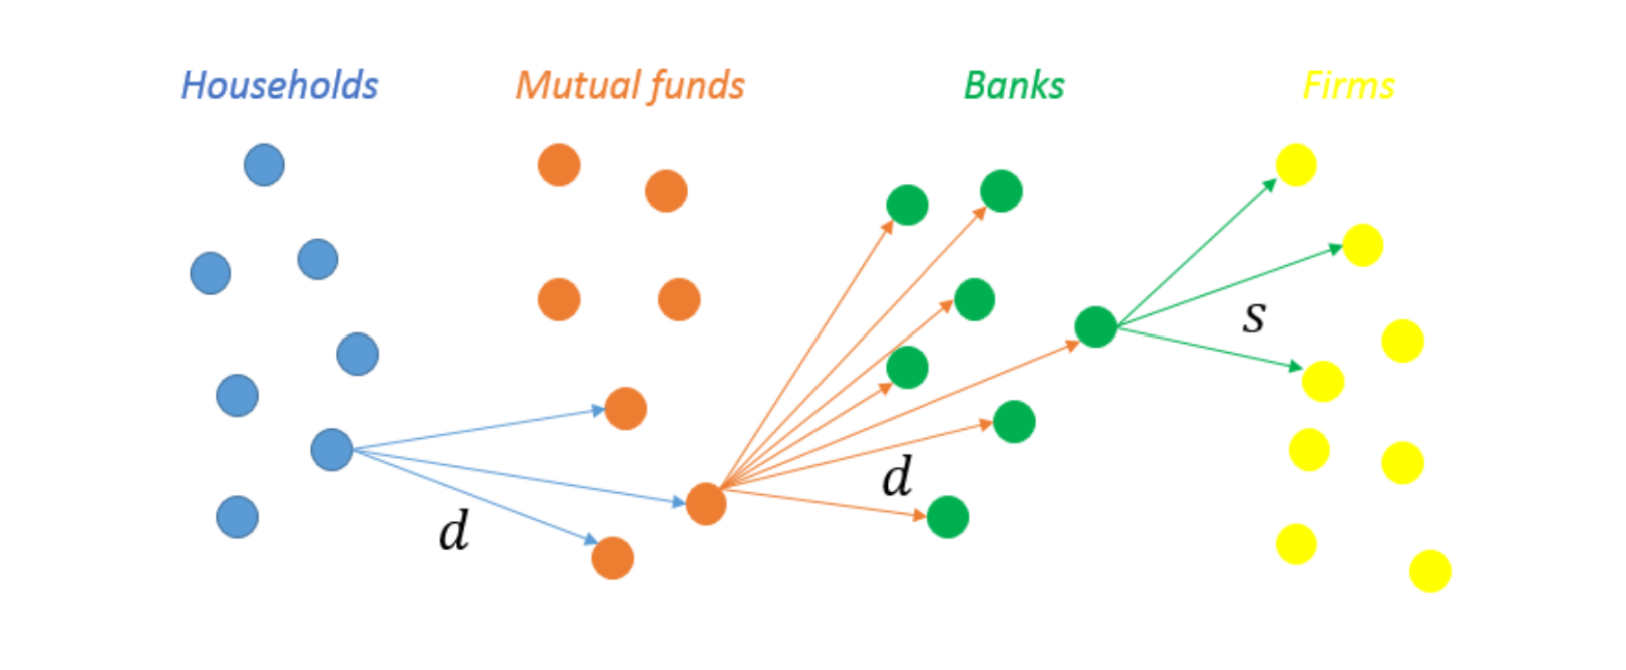
\includegraphics[width=\textwidth]{figures/HHK-lending.png}
    \caption{Household lending to banks}
\end{figure}
Entrepreneurs's net worth is:
\[
N_{t+1} = \gamma \int (\Pi_i )_t d i + W_t^e
\]
where $\Pi_i$ is entrepreneur $i$'s profits, $W_t^e$ is the entrepreneurs' labor income, $\gamma$ is the probability of not dying.

For HHs, they are like in the standard RBC model, with capital(return $R_{t+1}$).

Entrepreneurs’ output $Y_t$ is sold to the retail sector firms,
which are like the monopolistically competitive firms in the
NK model (with Calvo prices etc) and who turn this into a the
households’ consumption goods $c(i)$. Households as in NK
model.

\subsection{What do we get from all this?}

\begin{remark}[Financial accelerator mechanism]
    \ 

    Consider a negative demand shock to the economy,

    $\rightarrow$ reduces the quantity(or price $Q_t$) of output firms can sell

    $\rightarrow$ reduces the $MPK$ and Firm $i$'s asset value of holding capital $K$
    
    $\rightarrow$ reduces the net worth of entrepreneurs $N$

    $\rightarrow$ reduces the amount of capital entrepreneurs can borrow $QK-N$

    $\rightarrow$ reduces the amount of capital entrepreneurs can use in future investments

    $\rightarrow$ increases the external finance premium $s$

    $\rightarrow$ reduces investment and aggregate demand
\end{remark}

\subsubsection{Further analysis}

If you have a channel of how an asset price shock will be amplified,
you get even more amplification:

\underline{\textcolor{blue}{Bnak capital channel}}

Banks have to maintain a particular
maximum leverage ratio (size of the balance sheet vs. core
capital), which is Basel I, II, III.

If the value of your assets decrease, you have to write it off;
capital requirements will not be met anymore.

You have to sell off assets. This, in turn, reduces asset prices
(pecuniary externality).

Then the value of your assets decreases again.

\begin{definition}[Margin/Haircut spiral]
    \

    In times of crisis, banks increase 'haircuts',
    i.e. crisis $\Rightarrow$ value assets as a collateral less $\Rightarrow$ tightens borrowing
    constraint further
\end{definition}